\section{Problem Formulation}
\label{sec:problemformulation}

% Introduce the content of this section
The objective of the mesh network deployment is to minimize the number of 
deployed mesh nodes with the constraint of full coverage of the target area 
and connectivity to the Internet.  
In this section we first describe the the motivation, 
then we introduce the depolyment constraints, which
the QoS requirements of the vendors and clients.
Further, we formulate the deployment problem as a graph-theoretic model
with the QoS constraints. 

\subsection{Motivation}
\label{subsec:motivation}
% Propagation
Wireless propagation is the behavior of the signal loss characteristics 
when wireless signals are transmitted through the wireless medium.
The strength of the received signal depends on both the line-of-sight
path (or lack thereof) and multiple other paths that result from 
reflection, diffraction, and scattering from 
obstacles~\cite{andersen1995propagation}. The widely-used Friis
equation characterizes the received signal power $P_r$ in terms 
of transmit power $P_t$, transmitter gain $G_t$, receiver gain $G_r$, 
wavelength $\lambda$ of the carrier frequency, 
distance $R$ from transmitter to receiver, and path loss exponent 
$n$ according to~\cite{friis}:
\begin{equation}
\label{eq:friis}
P_r=P_t+G_t+G_r+10n \log_{10}\left( \frac{\lambda}{4\pi R}\right)
\end{equation}
Here, $n$ varies according to the aforementioned environmental 
factors with the value of two to five in typical outdoor 
settings~\cite{rappaport}. 
Through the propagation model, in the same environment with a 
constant pathloss exponent $n$, lower frequency white space 
bands offer not only more bandwidth, but also large communication
range, which could potentialy be used to reduce the number of 
access points.

Beamforming is a technique signals received at each antenna element are intelligently 
combined to improve the performance of the wireless system~\cite{winters2006smart}. 
As shown in Fig.~\ref{fig:aprange}, with the same transmit power, beamforming technology
could propagate the energy in directional lobe with a larger communication range.
Other than increasing communication range, beamforming could also potentially be used to 
suppress interfering signals, combat signal fading, and increase the capacity of 
wireless systems~\cite{bazan2012survey}. However, applying beamforming technology,
an access point could not reponse the request out of the beam lobes, which increase
the transmission time. The performance of throughput will be lower.

\begin{figure}
%\vspace{-0.0in}
\centering
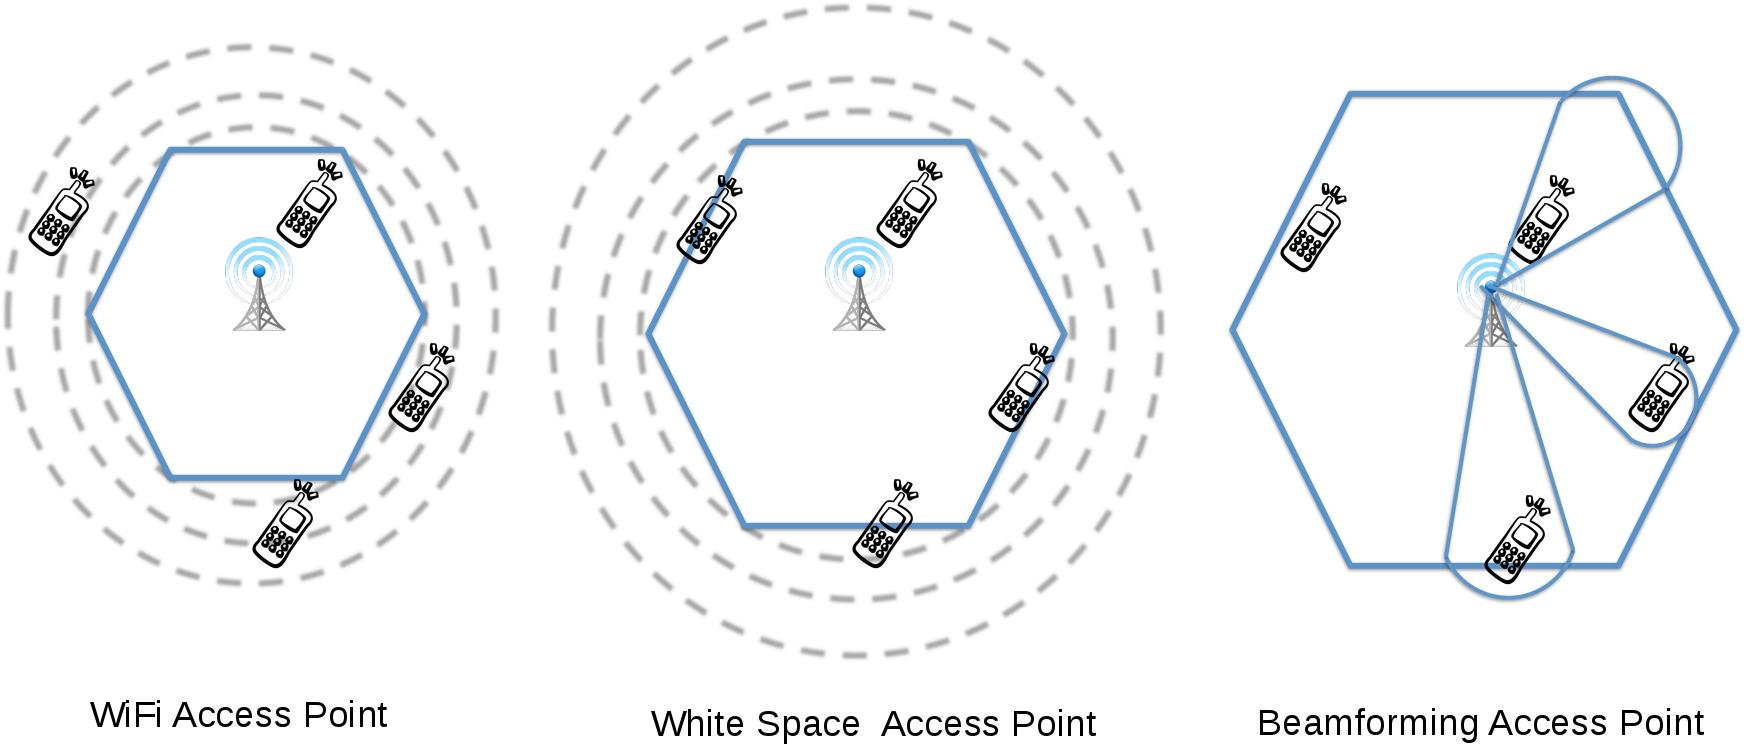
\includegraphics[width=84mm]{figures/com_range}
\vspace{-0.1in}
\caption{Communication Range of Access Points}                                                                 
\label{fig:aprange}
\vspace{-0.1in}
\end{figure}

Combine both beamforming and white space bands could expand a 
single mesh node coverage region 
and adapt the natural non-uniform 
traffic demand distribution 
The decrease of access points number means huge budget saving
in a wireless network deployment.

% Network Constraints
Typically, the deployment of wireless access networks is subject to coverage and capacity
constraints for a target area. Coverage is defined with respect to the ability of
clients to connect to access points within their service area.  We use a coverage
constraint ratio of $95\%$ in this work for a target area~\cite{robinson2010deploying}.
Capacity is defined with respect to the ability of a network to serve the traffic 
demand of clients.  Spatial reuse allows improved capacity, but increases the cost
of deploying a network by increasing the total number of access points required.
Hence, for densely populated areas the greatest level of spatial reuse possible
is often desired which could be offered through an expensive new access point working 
in other frequency or low cost beamforming with smart scheduling.
In contrast, sparsely-populated rural areas have lower traffic demand per unit area. Thus, 
aggregating this demand with lower-frequency, white space bands and further propagated beamforming
lobes could be highly effective in reducing the total number of access points required to achieve 
similar coverage and capacity constraints. 
Moreover, since less TV channels tend to be occupied in sparsely 
populated areas~\cite{msdatabase}, a larger number 
 of white space bands can be leveraged in these areas. 

% More variation in population distribution



\subsection{Model and Problem Formulation}
\label{subsec:problem}

% Assumptions of the network
As opposed to previous works such as~\cite{franklin2007node,robinson2010deploying
,si2010overview}, we focuse on hetergenous beamforming access point selection 
for wireless access networks which jointly employ white space and beamforming technology.
Through beamforming and white space agility, an access point performance could be
improve by the coverage area and throughput. Also with a smart beamforming scheduling, 
fairness in a network could be achieved through QoS time distribution.


We assume the service vendor has a limited number of spectrum resources and 
wireless radios have similar configuration, such as transmit power, gains and beam lobes. 
Each radio on an access point operates with a classic protocol model~\cite{gupta2000capacity}. 
Then we can further analyze the performance of access point under different 
traffic demand distribution according to the capacity 
and coverage constraint.

% Capacity constraint
A network deployment should ideally provide network capacity equal to the demand of the service 
area to maintain the capacity constraint. The demand of a service area could be calculated as the 
summation of individual demands all over the service area $D_a=\sum_{p\in P}D_p$. Since 
household demand for Internet has been previously characterized~\cite{rosston2011household}, 
$D_a$ could represent the population distribution $f$ and service area $k$ as 
$D_a=\sum_{f \in F,k \in K}\bar{D_p}*f*k$. 
The capacity constraint could be represented with access points set $M$ according to:
\begin{equation}
\label{eq:nlbound}
\sum_{m \in M}C_r^m \ge \sum_{f \in F,k \in K}\bar{D_p}*f*k
\end{equation}
% Coverage constraint
At the same time, the wireless network must additionally satisfy the coverage constraint in the service 
area where the access points provide connectivity for client devices. 
Generally, a coverage of $95\%$ is acceptable for wireless access networks~\cite{robinson2010deploying}.
The object of this work is to find the best possible number of access points so that the network has good 
connectivity and enough capacity to satisfy the traffic demands.

% Single beamforming access point service analysis
Under the capacity and coverage constraints, the serveice area of an access point 
is limited by the propagation range, beamforming lobes and scheduling methods. 
The radius of service area $r_s$ could be represented as:
\begin{equation}
\label{eq:servicearea}
r_s=min\{r_p,r_c\}
\end{equation}
$r_p$ represents the propagation range of the access point, $r_c$ is the capacity range of 
a radio in the access point. A simple example is when the traffic demand is distributed uniform in a circle, from 
Eq.~\ref{eq:nlbound} the capacity range $r_c$ could be noted as $r_c=\sqrt{k/\pi}$. 
Under beamforming situation, the capacity range $r_c$ will vary according to the 
beam lobe scheduling.
Moreover, the propagation range and capacity rang could be determined by the environment, traffic distribution and
power control~\cite{robinson2010deploying}. 
These parameters could be pre-detected from existing measurements, census and public or private database.
When a target area is given, we could model the traffic demand, access points and
potential connectivity links as a graph according to the parameters from database.


% Problem
Thus, the target area with pre-defined parameters could be modeled as a connectivity graph with 
vertexes represented as the centrilized traffic demand of a certain area and potential access points
locations. The edges note the links between the locations. 
Oppose to previous works,~\cite{robinson2010deploying,franklin2007node,tang2005interference,}
we formulate the input connectivity graph as a $3$ dimension graph $G = (V,E,F)$, where centralized
traffic demand, access points location candidates and links with or without beamforming form a
unified connectivity graph. 

The vertexes in the modeled input graph represent a set $C$ of  separated target area with traffic demands.
The set $C$ consists of physical coordinates represetnting target areas where client coverage is 
desired, analogous to the area to be covered in a geometric formulation and the traffic amount
need to be served.
And also the set of potential access points $M$ is a second part of the vertexes in the 
modeled graph. The potential locations of access points are assumed known through the 
infrastructure conditions.
The vertex set of the input connectivity graph is the union of potential access points
and centralized traffic demand locations as $V = C\cup M$.

The output of the problem is expected to be an graph $G' = (V',E',F')$ which marks the access points
and chosen links with/without beamforming. The connectvity and capacity constraints 
 

 
The nodes in the graph assume traffic demands of the target area could be discreted 
into a set $C$. The set $C$ consists of physical coordinates representing 
where coverage is desired, analogous to the area to be covered in a geometric formulation.

Previous work focus on the non-uniform coverage regions generated by environment. then find the 
solution to deploy minimum number of access points. In this work, we use frequency agility and 
beamforming to generate non-uniform coverage regions to reduce the number of access points
for a network deployment.

To do that...


